\chapter{$1s$原初高斯函数的积分计算方法}
\label{appendix:a}


大多数分子计算使用固定的分子坐标系,使得基函数以该坐标系中的位置矢量
$\bo{R}_A$为中心,如\autoref{figA.1}所示。一个以$\bo{R}_A$为中心的
位置矢量$\bo{r}$的值将会依赖于$\bo{r}-\bo{R}_A$,因此我们可以写一个一般化的基函数
$\phi_\mu(\bo{r}-\bo{R}_A)$来代表它是以$\bo{R}_A$为中心的。在一个分子计算的过程中
我们需要计算数量庞大的包含不同中心$\phi_\mu(\bo{r}-\bo{R}_A)$的单电子和双电子积分。
如果我们使用的基函数包括四个或者更多的中心,那么我们的双电子积分将会包含$1-$、$2-$、$3-$和
$4-$中心积分。核吸引势积分最多只能处理到三中心。这些多中心(超过$2$)的积分对于Slater型函数
来说非常难以处理,但是对于Gaussian型函数来说处理起来相对简单。因此许多多原子计算使用Gaussian函数。
\begin{figure}[h]
	\begin{tikzpicture}[scale=2,inner sep=0,arrows=-latex]
		\draw (0,0)--(0,2);
		\draw (0,0)--(-1.2,-1.2);
		\draw (0,0)--(2,0);
		\draw (2,1) circle[radius=0.3];
		\node (A) at (2,1) {\bf A};
		\node (i) at (.7,1.8) {} ;
		\fill (i) circle(1pt) ;
		\draw (0,0)--node[right=13pt]{$\mathbf{R_A}$}(A);
		\draw (0,0)--node[right=5pt]{$\mathbf{r}$}(i);
		\draw (A)--node[right=.2cm]{$\mathbf{r-R_A}$}(i);
	\end{tikzpicture}
	\caption{分子坐标系}
	\label{figA.1}
\end{figure}

在高斯函数的计算中,收缩型的高斯基函数$\phi_\mu^{CGF}$一般由一系列的原初高斯函数
$g\equiv\phi_p^{GF}$(见\autoref{3.283}或\autoref{3.212}) 展开,因此我们只需要考虑
计算这些原初函数之间的积分即可。收缩函数$\phi_\mu^{CGF}$的积分只需要通过对原初函数的积分
用恰当的收缩系数进行求和就能得到。一般常用$1s$、$2p$、$3d$等原初高斯函数,因为任何$s$、$p$、
$d$的函数能够类似的用这些高斯函数展开。这里我们仅考虑$1s$原初高斯函数积分的计算。
Shavitt 
\endnote{I.Shavitt,The Gaussian function in calculations of statistical mechanics and quantummechanics,in \textit{Methods in Computational Physics}
,B.Aledr,S.Fernbach,and M.Rotenberg (Eds.),Academic Press,New York,1963.}
已经给出了一个相似的但是可以互通有无的关于高斯函数积分计算的讨论。包含$p$、$d$等类似函数的积分
可以通过把我们结果对中心$\bo{R}_A$、$\bo{R}_B$等在笛卡尔坐标系中的坐标进行微分得到。但是,
高角量子数的积分计算通过基于Rys多项式的新方法更高效的实现。\endnote{
M. Dupuis,J. Rys,and H. King,Evaluation of molecular integrals over Gaussian basis functions,\textit{J. Chem. Phys.} \textbf{65}:111 (1976).}

以$\bo{R}_A$未归一化的$1s$原初高斯函数为
\begin{align}
	\label{A.1}
	\tilde{g}_{1s}(\bo{r}-\bo{R}_A)=e^{-\alpha\lvert \bo{r}-\bo{R}_A \rvert ^2}
\end{align}
我们将用$\alpha$、$\beta$、$\gamma$和$\delta$分别表示$\bo{R}_A$、
$\bo{R}_B$、$\bo{R}_C$、$\bo{R}_D$的轨道指数。高斯函数能够简化多中心电子积分的原因是
两个不同中心的$1s$高斯函数的乘积可以成比例的化成1个在第三个中心的$1s$高斯函数。因此
\begin{align}
	\label{A.2}
	\tilde{g}_{1s}(\bo{r}-\bo{R}_A)\tilde{g}_{1s}(\bo{r}-\bo{R}_B)
	=\tilde{K}\tilde{g}_{1s}(\bo{r}-\bo{R}_P)
\end{align}
其中,比例系数$\tilde{K}$为
\begin{align}
	\label{A.3}
    \tilde{K}=\exp[-\alpha\beta/(\alpha+\beta)\lvert \bo{R}_A-\bo{R}_B \rvert ^2]
\end{align}
第三个中心$P$落在中心$A$和$B$的连线上,
\begin{align}
	\label{A.4}
	\bo{R}_P=(\alpha\bo{R}_A+\beta \bo{R}_B)/(\alpha+\beta)
\end{align}
中心在$\bo{R}_P$的新高斯函数的指数为
\begin{align}
	\label{A.5}
	p=\alpha+\beta
\end{align}
因此对于$1s$高斯函数的任何2-中心分布,例如,两个不同中心的函数的乘积,能够马上转化成一个单中心
分布的高斯函数。我们现在计算任何从头算计算过程都需要的仅收缩$1s$原初高斯函数的基本积分。我们将
计算未归一化的函数的积分,并且如果我们需要归一化的函数的积分,我们可以简单的乘一个合适的归一化
常数来得到它。

首先考虑2-中心的重叠积分
\begin{align}
	\label{A.6}
	(A|B)=\int \emph{d}\bo{r}_1\,\tilde{g}_{1s}(\bo{r}_1-\bo{R}_A)\tilde{g}_{1s}(\bo{r}_1-\bo{R}_B)
\end{align}
通过\autoref{A.2},我们马上得到
\begin{align}
	\label{A.7}
	(A|B)=\tilde{K}\int \emph{d}\bo{r}_1\,\tilde{g}_{1s}(\bo{r}_1-\bo{R}_P)
	=\tilde{K}\int \emph{d}\bo{r}_1\, \exp[-p\lvert \bo{r}_1-\bo{R}_P \rvert ^2]
\end{align}
如果我们使$\bo{r}=\bo{r}_1-\bo{R}_p$并且$\emph{d}\bo{r}\,=\emph{d}\bo{r}_1\,$,则
\begin{align}
	\label{A.8}
	(A|B)=\tilde{K}\int \emph{d}\bo{r}\,\,e^{-p\bo{r}^2}=4\pi\tilde{K}\int_0^{\infty} \emph{d}r\,r^2e^{-pr^2}
\end{align}
最后一个积分的值恰好是$(\pi/p)^{\frac{3}{2}}/{4\pi}$,所以
\begin{align}
	\label{A.9}
	(A|B)=[pi/(\alpha+\beta)]^{\frac{3}{2}}\exp[-\alpha\beta/(\alpha+\beta)\lvert \bo{R}_A-\bo{R}_B \rvert ^2]
\end{align}

动能积分为
\begin{align}
	\label{A.10}
	(A|-\frac{1}{2}\nabla^2|B)=\int \emph{d}\bo{r}_1\,\tilde{g}_{1s}(\bo{r}_1-\bo{R}_A)(-\frac{1}{2}\nabla_1^2)\tilde{g}_{1s}(\bo{r}_1-\bo{R}_B)
\end{align}
在算符$\nabla_1^2$作用完成后,上式能够通过非常类似的方式进行计算,得到
\begin{align}
	\label{A.11}
	(A|-\frac{1}{2}\nabla^2|B)=&\alpha\beta/(\alpha+\beta)[3-2\alpha\beta/(\alpha+\beta)\lvert \bo{R}_A-\bo{R}_B \rvert ^2][\pi/(\alpha+\beta)]^{\frac{3}{2}}\nonumber\\
	&\times\exp[-\alpha\beta/(\alpha+\beta)\lvert \bo{R}_A-\bo{R}_B \rvert ^2]
\end{align}

为了计算核吸引势能积分和双电子排斥积分,现在我们在这里介绍一种强力的并常用的,对于计算积分
尤其是我们将要讨论的类型的积分往往有效的方法。这种方法是将每一个我们需要积分的变量替换为它的
傅里叶变换的形式。如果我们给定了一个矢量$\bo{r}$的函数$f(\bo{r})$,那么它的三维坐标傅里叶变换
$F(\bo{k})$定义为
\begin{align}
	\label{A.12}
	F(\bo{k})=\int \emph{d}\bo{r}\,f(\bo{r})e^{-i\bo{k}\bo{r}}
\end{align}
其中矢量$\bo{k}$是变换变量。傅里叶积分定理说明
\begin{align}
	\label{A.13}
	f(\bo{r})=(2\pi)^{-3}\int \emph{d}\bo{k}\,F(\bo{k})e^{i\bo{k}\bo{r}}
\end{align}
\begin{table}[h!] 
	
	\caption{Fourier transform pairs}
	\centering
	\begin{tabular}{lll}
		\hline 
		$f(\bm{r})$ & ~~~~ ~~~~& $F(\bm{k})$ \\ \hline \\
		$\frac{1}{r}$&  ~~~~ ~~~~& $\frac{4\pi}{k^2}$ \\
		\\
		$e^{-\alpha^2}$ & ~~~~ ~~~~ & $(\frac{\pi}{\alpha})^{\frac{3}{2}}e^{-k^2/{4\alpha}}$\\
		\\
		$\delta(\bo{r})$& ~~~~ ~~~~ &1
	\\ \hline
	\end{tabular}
	\label{tA.1}
\end{table}
$F(\bo{k})$和$f(\bo{r})$被称为一个傅里叶变换对。所有的我们将要用到的傅里叶变换对都在
\autoref{tA.1}给出。特别的,傅里叶表示下的三维坐标狄拉克$delta$函数是
\begin{align}
	\label{A.14}
	\delta(\bo{r}_1-\bo{r}_2)=(2\pi)^{-3}\int \emph{d}\bo{k}\,F(\bo{k})e^{i\bo{k}(\bo{r}_1-\bo{r_2})}
\end{align}

正如之前提到的,狄拉克$\delta$函数有以下性质
\begin{align}
	\label{A.15}
	\int \emph{d}\bo{r}_1\,\delta(\bo{r}_1-\bo{r}_2)h(\bo{r}_1)=h(\bo{r}_2)
\end{align}
上式对于任意一个函数$h(\bo{r})$都成立。

让我们现在考虑$1s$原初高斯函数的核吸引势积分,
\begin{align}
	\label{A.16}
	(A|-Z_C/r_{1C}|B)=&\int\emph{d}\bo{r}_1\,\tilde{g}_{1s}(\bo{r}_1-\bo{R}_A)
	[-Z_C/|\bo{r}_1-\bo{R}_C|^{-1}]\tilde{g}_{1s}(\bo{r}_1-\bo{R}_B) \nonumber\\
	=&-Z_C\int\emph{d}\bo{r}_1\,e^{-\alpha\lvert \bo{r}-\bo{R}_A \rvert ^2}|\bo{r}_1-\bo{R}_C|^{-1}
	e^{-\beta\lvert \bo{r}-\bo{R}_B \rvert ^2}
\end{align}
我们首先把两个高斯函数结合,得到一个中心在$\bo{R}_P$的高斯函数,
\begin{align}
	\label{A.17}
	(A|-Z_C/r_{1C}|B)=-Z_C\tilde{K}\int\emph{d}\bo{r}_1\,e^{-p\lvert \bo{r}-\bo{R}_P \rvert ^2}|\bo{r}_1-\bo{R}_C|^{-1}
\end{align}
然后,我们用\autoref{A.13}和\autoref{tA.1}中的变换形式替换上面的两项,
\begin{align}
	\label{A.18}
	(A|-Z_C/r_{1C}|B)=&-Z_C\tilde{K}(2\pi)^{-6}(\pi/p)^{3/2}
	\int\emph{d}\bo{r}_1\emph{d}\bo{k}_1\emph{d}\bo{k}_2\,e^{-\bo{k}_1^2/4p}\nonumber\\
	&\times e^{i\bo{k}_1\cdot(\bo{r}_1-\bo{R}_P)}4\pi k_2^{-2}e^{i\bo{k}_2\cdot(\bo{r}_1-\bo{R}_C)}
\end{align}
如果我们合并所有含有原来积分变量$\bo{r}_1$的指数项,我们得到
\begin{align}
	\label{A.19}
	(A|-Z_C/r_{1C}|B)=&-4\pi Z_C\tilde{K}(2\pi)^{-6}(\pi/p)^{3/2}
	\int\emph{d}\bo{r}_1\emph{d}\bo{k}_1\emph{d}\bo{k}_2\,k_2^{-2}e^{-\bo{k}_1^2/4p}\nonumber\\
	&\times e^{-i\bo{k}_1\cdot\bo{R}_P}e^{-i\bo{k}_2\cdot\bo{R}_C}e^{i\bo{r}_1\cdot(\bo{k}_1+\bo{k}_2)}
\end{align}
我们现在可以用\autoref{A.14}定义的$\delta$函数处理$\bo{r}_1$的积分,得到
\begin{align}
	\label{A.20}
	(A|-Z_C/r_{1C}|B)=&-4\pi Z_C\tilde{K}(2\pi)^{-3}(\pi/p)^{3/2}
	\int\emph{d}\bo{k}_1\emph{d}\bo{k}_2\,e^{-\bo{k}_1^2/4p}k_2^{-2}\nonumber\\
	&\times e^{i\bo{k}_1\cdot\bo{R}_P}e^{-i\bo{k}_2\cdot\bo{R}_C}\delta(\bo{k}_1+\bo{k}_2)\nonumber\\
	&=-Z_C\tilde{K}(2\pi^{2})(\pi/p)^{3/2}\int\emph{d}\bo{k}\,e^{-\bo{k}^2/4p}k^{-2} e^{-i\bo{k}\cdot(\bo{R}_P-\bo{R}_C)}
\end{align}
由于$\delta$函数的存在,这里我们令$\bo{k}_2=-\bo{k}_1$,并且重新把变量记为$\bo{k}$。如果我们
令$\bo{R}_P-\bo{R}_C$落在$z$轴上,那么$\bo{k}\cdot(\bo{R}_P-\bo{R}_C)=k|\bo{R}_P-\bo{R}_C|\cos(\theta)$,
之后我们可以简单的处理角度部分在$\bo{k}$上的积分,
\begin{align}
	\label{A.21}
	(A|-Z_C/r_{1C}|B)=&N\int^{\infty}_0\emph{d}k\,e^{-\bo{k}^2/4p}k^{-1}\sin{(k|\bo{R}_P-\bo{R}_C|)}
\end{align}
\begin{align}
	\label{A.22}
	N=-2Z_C\tilde{K}(\pi |\bo{R}_P-\bo{R}_C|)^{-1}(\pi/p)^{3/2}
\end{align}
为了计算\autoref{A.21}中的积分,我们考虑下列一般化的积分:
\begin{align}
	\label{A.23}
	I(x)=\int^{\infty}_0\emph{d}k\,e^{-a k^2}k^{-1}\sin{kx}
\end{align}
上式对$x$的导数为
\begin{align}
	\label{A.24}
	I`(x)=\int^{\infty}_0\emph{d}k\,e^{-a k^2}\cos{kx}
\end{align}
注意\autoref{A.24}是$k$的偶函数。由于$I(0)=0$,我们得到
\begin{align}
	\label{A.25}
	\int^{x}_0 \emph{d}yI`(y)=I(x)-I(0)=I(x)
\end{align}
注意到$\cos(\theta)$是$e^{i\theta}$的实数部分(例如,$\cos(\theta)=\Re e[e^{i\theta}]$),
\autoref{A.24}中的积分可以这样来计算
\begin{align}
	\label{A.26}
	I`(x)=\frac{1}{2}\int^{\infty}_{-\infty}\emph{d}k\,e^{-a k^2}\cos{kx}=\frac{1}{2}\Re e\biggl[\int^{\infty}_{-\infty}\emph{d}k\,e^{-a k^2}e^{ikx}\biggr]
\end{align}
通过凑平方,我们得到
\begin{align}
	\label{A.27}
	I`(x)=\frac{1}{2}e^{-x^2/4a}\Re e\biggl[\int^{\infty}_{-\infty}\emph{d}k\,e^{-(a^{1/2}k-1/2i a^{-1/2}x)^2}\biggr]
\end{align}
令$u=a^{1/2}k-1/2i a^{-1/2}x$,我们得到
\begin{align}
	\label{A.28}
	I`(x)=\frac{1}{2}e^{-x^2/4a}a^{-1/2}\int^{\infty}_{-\infty}\emph{d}u\,e^{-u^2}=\frac{1}{2}(\pi /a)^{1/2}e^{-x^2/4a}
\end{align}
故
\begin{align}
	\label{A.29}
	I(x)=\frac{1}{2}(\pi /a)^{1/2}\int^{x}_{0}\emph{d}ye^{-y^2/4a}
\end{align}
因此
\begin{align}
	\label{A.30}
	(A|-Z_C/r_{1C}|B)=&-2\pi Z_C\tilde{K}(p|\bo{R}_P-\bo{R}_C|)^{-1}\int^{|\bo{R}_P-\bo{R}_C|}_{0}\emph{d}y\,e^{-py^2}
\nonumber\\
	=&-2\pi Z_C\tilde{K}p^{-1}(p^{1/2}|\bo{R}_P-\bo{R}_C|)^{-1}\int^{p^{1/2}|\bo{R}_P-\bo{R}_C|}_{0}\emph{d}y\,e^{-y^2}
\end{align}
我们现在引入$F_0$函数,定义为
\begin{align}
	\label{A.31}
	F_0(t)=t^{-1/2}\int_0^{t^{1/2}}\emph{d}y\,e^{-y^2}
\end{align}
它可以通过下式与误差函数关联起来
\begin{align}
	\label{A.32}
	F_0(t)=\frac{1}{2}(\pi/t)^{1/2}erf(t^{1/2})
\end{align}
因此,我们的核吸引势积分可以写成包含$F_0$的形式
\begin{align}
	\label{A.33}
	(A|-Z_C/r_{1C}|B)=&-2\pi/(\alpha+\beta) Z_C\exp[-\alpha\beta/(\alpha+\beta)|\bo{R}_A-\bo{R}_B|^2]
	\nonumber\\
	\times&F_0[(\alpha+\beta)|\bo{R}_P-\bo{R}_C|^2]
\end{align}
误差函数(在这里是$F_0$)是一个IBM FORTRAN编译器里的内置函数。

我们现在开始考虑双电子积分
\begin{align}
	\label{A.34}
	(AB|CD)=\int\emph{d}\bo{r}_1\emph{d}\bo{r}_2\,\tilde{g}_{1s}(\bo{r}_1-\bo{R}_A)
	\tilde{g}_{1s}(\bo{r}_1-\bo{R}_B)r_{12}^{-1}\tilde{g}_{1s}(\bo{r}_2-\bo{R}_C)\tilde{g}_{1s}(\bo{r}_2-\bo{R}_D)
\end{align}
第一步是将中心在$\bo{R}_A$和$\bo{R}_B$的高斯函数合并成一个新的、中心在$\bo{R}_P$高斯函数,
以及将中心在$\bo{R}_C$和$\bo{R}_D$的高斯函数合并成一个新的、中心在$\bo{R}_Q$高斯函数,如
\autoref{figA.2}所示,则\autoref{A.34}化为
\begin{align}
	\label{A.35}
	(AB|CD)=&\exp[-\alpha\beta/(\alpha+\beta)|\bo{R}_A-\bo{R}_B|^2-\gamma\delta/(\gamma+\delta)|\bo{R}_C-\bo{R}_D|^2]
	\nonumber\\
	\times&\int\emph{d}\bo{r}_1\emph{d}\bo{r}_2\,e^{-p\lvert \bo{r}_1-\bo{R}_P \rvert ^2}r_{12}^{-1}e^{-q\lvert \bo{r}_2-\bo{R}_Q \rvert ^2}
\end{align}

\begin{figure}[h]
	\begin{tikzpicture}[scale=2,inner sep=0,arrows=-latex]
		\draw (0,0)--(0,2);
		\draw (0,0)--(-1.2,-1.2);
		\draw (0,0)--(2,0);
		\coordinate(a) at(0.9,1.4);
		\coordinate(b) at(0.5,0.3);
		\coordinate(c) at(1.4,1.4);
		\coordinate(d) at(1.9,0.25);
		\node (A) at (1,1.5) {\bf A};
		\node (B) at (0.6,0.2) {\bf B};
		\node (C) at (1.5,1.5) {\bf C};
		\node (D) at (2,0.15) {\bf D};
		\fill (a) circle(1pt) ;
		\fill (b) circle(1pt) ;
		\fill (c) circle(1pt) ;
		\fill (d) circle(1pt) ;
		\draw (a) -- (b);
		\draw (c) -- (d);
		\coordinate(p) at(0.6,0.575);
		\node (P) at (0.47,0.6) {\bf P};
		\fill (p) circle(1pt) ;
		\coordinate(q) at(1.5,1.17);
		\node (Q) at (1.6,1.2) {\bf Q};
		\fill (q) circle(1pt) ;
		\draw (p)--node[below=0.4cm]{$\mathbf{R_Q-R_P}$}(q);
	\end{tikzpicture}
	\caption{双电子积分中包含的六个中心}
	\label{figA.2}
\end{figure}
把积分中的三项替换为它们的傅里叶变换形式,得
\begin{align}
	\label{A.36}
	(AB|CD)=&M(2\pi)^{-9}\int\emph{d}\bo{r}_1\emph{d}\bo{r}_2\emph{d}\bo{k}_1\emph{d}\bo{k}_2\emph{d}\bo{k}_3\,
	(\pi/p)^{3/2}e^{-k_1^2/{4p}}e^{i\bo{k}_1\cdot(\bo{r}_1-\bo{R}_P)}
	\nonumber\\
	\times&4\pi k_2^{-2}e^{i\bo{k}_2\cdot(\bo{r}_1-\bo{r}_2)}
	(\pi/q)^{3/2}e^{-k_3^2/{4q}}e^{i\bo{k}_3\cdot(\bo{r}_2-\bo{R}_Q)}
\end{align}
其中
\begin{align}
	\label{A.37}
	M=\exp[-\alpha\beta/(\alpha+\beta)|\bo{R}_A-\bo{R}_B|^2-\gamma\delta/(\gamma+\delta)|\bo{R}_C-\bo{R}_D|^2]
\end{align}
把初始变量$\bo{r}_1$和$\bo{r}_2$的指数项合并,得到
\begin{align}
	\label{A.38}
	(AB|CD)=&4\pi M(2\pi)^{-9}(\pi^2/p)q^{3/2}\int\emph{d}\bo{r}_1\emph{d}\bo{r}_2\emph{d}\bo{k}_1\emph{d}\bo{k}_2\emph{d}\bo{k}_3\,
	e^{-k_1^2/{4p}}e^{-k_3^2/{4q}}
	\nonumber\\
	\times&k_2^{-2}e^{-i\bo{k}_1\cdot\bo{R}_P}e^{-i\bo{k}_3\cdot\bo{R}_Q}e^{i\bo{r}_1\cdot(k_1+k_2)}
	e^{i\bo{r}_2\cdot(k_3-k_2)}
\end{align}
现在对在$\bo{r}_1$和$\bo{r}_2$上的积分引入两个delta函数\autoref{A.14}
\begin{align}
	\label{A.39}
	(AB|CD)=&4\pi M(2\pi)^{-9}(\pi^2/p)q^{3/2}\int\emph{d}\bo{k}_1\emph{d}\bo{k}_2\emph{d}\bo{k}_3\,
	e^{-k_1^2/{4p}}e^{-k_3^2/{4q}}
	\nonumber\\
	\times&k_2^{-2}e^{-i\bo{k}_1\cdot\bo{R}_P}e^{-i\bo{k}_3\cdot\bo{R}_Q}
	\delta(k_1+k_2)\delta(k_3-k_2)
\end{align}
现在我们令$k_1=-k_2$和$k_3=k_2$,并重新把$k_2$记为$k$,得
\begin{align}
	\label{A.40}
	(AB|CD)=&4\pi M(2\pi)^{-9}(\pi^2/p)q^{3/2}\int\emph{d}\bo{k}\,
	k^{-2}e^{-(p+q)k^2/4pq}e^{i\bo{k}\cdot(\bo{R}_P-\bo{R}_Q)}
\end{align}
这个积分等同于我们在计算核吸引势积分时遇到的\autoref{A.20}的形式。进行剩余的代数过程
我们最终得到
\begin{align}
	\label{A.41}
	(AB|CD)=&2\pi ^{5/2}/[(\alpha+\beta)(\gamma+\delta)(\alpha+\beta+\gamma+\delta)^{1/2}]
	\nonumber\\
	\times&\exp[-\alpha\beta/(\alpha+\beta)|\bo{R}_A-\bo{R}_B|^2-\gamma\delta/(\gamma+\delta)|\bo{R}_C-\bo{R}_D|^2]
	\nonumber\\
	\times&F_0[(\alpha+\beta)(\gamma+\delta)(\alpha+\beta+\gamma+\delta)|\bo{R}_P-\bo{R}_Q|^2]
\end{align}
以上这些就是我们仅用$1s$类型的原初高斯函数进行Hartree-Fock计算所需要的所有积分的精确方程。
它们被用在附录B中计算机程序中。

\newpage
\theendnotes
\addcontentsline{toc}{section}{注释}


\begin{figure}[h]
	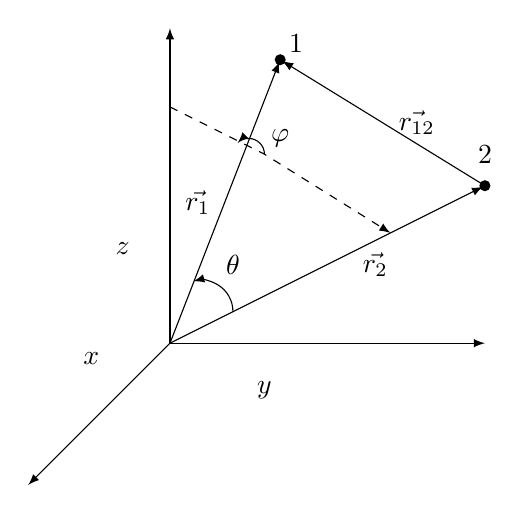
\begin{tikzpicture}[scale=2,inner sep=0,arrows=-latex]
		\draw  (0,0)--(0,2);
		\draw (0,0)--(-0.9,-0.9);
		\draw (0,0)--(2,0);
		\node (x) at (-0.5,-0.1) {\bf $x$};
		\node (y) at (0.6,-0.3) {\bf $y$};
		\node (z) at (-.3,0.6) {\bf $z$};
		% \draw (2,1) circle[radius=0.3];
		\node (A) at (2,1) {};
		\node (i) at (.7,1.8) {} ;
		\node (r1) at (2,1.2) {\bf $2$};
		\node (r2) at (.8,1.9) {\bf $1$} ;
		\fill (i) circle(1pt) ;
		\fill (A) circle(1pt) ;
		\draw (0,0)--node[right=13pt]{${\vec{{r_2}}}$}(A);
		\draw (0,0)--node[left=5pt]{${\vec{{r_1}}}$}(i);
		\draw (A)--node[right=.2cm]{${\vec{{r_{12}}}}$}(i);
		\draw [dashed,] (0,1.5) -- (.6,1.2) -- (1.4,0.7);
		\draw (0.6,1.2) arc (0:135:0.1);
		\node (phi) at (.7,1.3) {$\varphi$} ;
		% \draw[dashed] (0.1,0.05) -- (0.12,.2) -- (0.14,0.36);
		\draw (0.4,0.2) arc (0:105:0.2);
		\node (theta) at (.4,.5) {$\theta$} ;
	\end{tikzpicture}
	% \caption{分子坐标系}
	\label{figA.-1}
\end{figure}
\chapter{$1s$原初高斯函数的积分计算方法}
\label{appendix:a}


大多数分子计算使用固定的分子坐标系,使得基函数以该坐标系中的位置矢量
$\bo{R}_A$为中心,如\autoref{figA.1}所示。一个以$\bo{R}_A$为中心的
位置矢量$\bo{r}$的值将会依赖于$\bo{r}-\bo{R}_A$,因此我们可以写一个一般化的基函数
$\phi_\mu(\bo{r}-\bo{R}_A)$来代表它是以$\bo{R}_A$为中心的。在一个分子计算的过程中
我们需要计算数量庞大的包含不同中心$\phi_\mu(\bo{r}-\bo{R}_A)$的单电子和双电子积分。
如果我们使用的基函数包括四个或者更多的中心,那么我们的双电子积分将会包含$1-$、$2-$、$3-$和
$4-$中心积分。核吸引势积分最多只能处理到三中心。这些多中心(超过$2$)的积分对于Slater型函数
来说非常难以处理,但是对于Gaussian型函数来说处理起来相对简单。因此许多多原子计算使用Gaussian函数。
\begin{figure}[h]
	\begin{tikzpicture}[scale=2,inner sep=0,arrows=-latex]
		\draw (0,0)--(0,2);
		\draw (0,0)--(-1.2,-1.2);
		\draw (0,0)--(2,0);
		\draw (2,1) circle[radius=0.3];
		\node (A) at (2,1) {\bf A};
		\node (i) at (.7,1.8) {} ;
		\fill (i) circle(1pt) ;
		\draw (0,0)--node[right=13pt]{$\mathbf{R_A}$}(A);
		\draw (0,0)--node[right=5pt]{$\mathbf{r}$}(i);
		\draw (A)--node[right=.2cm]{$\mathbf{r-R_A}$}(i);
	\end{tikzpicture}
	\caption{分子坐标系}
	\label{figA.1}
\end{figure}

在高斯函数的计算中,收缩型的高斯基函数$\phi_\mu^{CGF}$一般由一系列的原初高斯函数
$g\equiv\phi_p^{GF}$(见\autoref{3.283}或\autoref{3.212}) 展开,因此我们只需要考虑
计算这些原初函数之间的积分即可。收缩函数$\phi_\mu^{CGF}$的积分只需要通过对原初函数的积分
用恰当的收缩系数进行求和就能得到。一般常用$1s$、$2p$、$3d$等原初高斯函数,因为任何$s$、$p$、
$d$的函数能够类似的用这些高斯函数展开。这里我们仅考虑$1s$原初高斯函数积分的计算。
Shavitt 
\endnote{I.Shavitt,The Gaussian function in calculations of statistical mechanics and quantummechanics,in \textit{Methods in Computational Physics}
,B.Aledr,S.Fernbach,and M.Rotenberg (Eds.),Academic Press,New York,1963.}
已经给出了一个相似的但是可以互通有无的关于高斯函数积分计算的讨论。包含$p$、$d$等类似函数的积分
可以通过把我们结果对中心$\bo{R}_A$、$\bo{R}_B$等在笛卡尔坐标系中的坐标进行微分得到。但是,
高角量子数的积分计算通过基于Rys多项式的新方法更高效的实现。\endnote{
M. Dupuis,J. Rys,and H. King,Evaluation of molecular integrals over Gaussian basis functions,\textit{J. Chem. Phys.} \textbf{65}:111 (1976).}

以$\bo{R}_A$未归一化的$1s$原初高斯函数为
\begin{align}
	\label{A.1}
	\tilde{g}_{1s}(\bo{r}-\bo{R}_A)=e^{-\alpha\lvert \bo{r}-\bo{R}_A \rvert ^2}
\end{align}
我们将用$\alpha$、$\beta$、$\gamma$和$\delta$分别表示$\bo{R}_A$、
$\bo{R}_B$、$\bo{R}_C$、$\bo{R}_D$的轨道指数。高斯函数能够简化多中心电子积分的原因是
两个不同中心的$1s$高斯函数的乘积可以成比例的化成1个在第三个中心的$1s$高斯函数。因此
\begin{align}
	\label{A.2}
	\tilde{g}_{1s}(\bo{r}-\bo{R}_A)\tilde{g}_{1s}(\bo{r}-\bo{R}_B)
	=\tilde{K}\tilde{g}_{1s}(\bo{r}-\bo{R}_P)
\end{align}
其中,比例系数$\tilde{K}$为
\begin{align}
	\label{A.3}
    \tilde{K}=\exp[-\alpha\beta/(\alpha+\beta)\lvert \bo{R}_A-\bo{R}_B \rvert ^2]
\end{align}
第三个中心$P$落在中心$A$和$B$的连线上,
\begin{align}
	\label{A.4}
	\bo{R}_P=(\alpha\bo{R}_A+\beta \bo{R}_B)/(\alpha+\beta)
\end{align}
中心在$\bo{R}_P$的新高斯函数的指数为
\begin{align}
	\label{A.5}
	p=\alpha+\beta
\end{align}
因此对于$1s$高斯函数的任何2-中心分布,例如,两个不同中心的函数的乘积,能够马上转化成一个单中心
分布的高斯函数。我们现在计算任何从头算计算过程都需要的仅收缩$1s$原初高斯函数的基本积分。我们将
计算未归一化的函数的积分,并且如果我们需要归一化的函数的积分,我们可以简单的乘一个合适的归一化
常数来得到它。

首先考虑2-中心的重叠积分
\begin{align}
	\label{A.6}
	(A|B)=\int \emph{d}\bo{r}_1\,\tilde{g}_{1s}(\bo{r}_1-\bo{R}_A)\tilde{g}_{1s}(\bo{r}_1-\bo{R}_B)
\end{align}
通过\autoref{A.2},我们马上得到
\begin{align}
	\label{A.7}
	(A|B)=\tilde{K}\int \emph{d}\bo{r}_1\,\tilde{g}_{1s}(\bo{r}_1-\bo{R}_P)
	=\tilde{K}\int \emph{d}\bo{r}_1\, \exp[-p\lvert \bo{r}_1-\bo{R}_P \rvert ^2]
\end{align}
如果我们使$\bo{r}=\bo{r}_1-\bo{R}_p$并且$\emph{d}\bo{r}\,=\emph{d}\bo{r}_1\,$,则
\begin{align}
	\label{A.8}
	(A|B)=\tilde{K}\int \emph{d}\bo{r}\,\,e^{-p\bo{r}^2}=4\pi\tilde{K}\int_0^{\infty} \emph{d}r\,r^2e^{-pr^2}
\end{align}
最后一个积分的值恰好是$(\pi/p)^{\frac{3}{2}}/{4\pi}$,所以
\begin{align}
	\label{A.9}
	(A|B)=[pi/(\alpha+\beta)]^{\frac{3}{2}}\exp[-\alpha\beta/(\alpha+\beta)\lvert \bo{R}_A-\bo{R}_B \rvert ^2]
\end{align}

动能积分为
\begin{align}
	\label{A.10}
	(A|-\frac{1}{2}\nabla^2|B)=\int \emph{d}\bo{r}_1\,\tilde{g}_{1s}(\bo{r}_1-\bo{R}_A)(-\frac{1}{2}\nabla_1^2)\tilde{g}_{1s}(\bo{r}_1-\bo{R}_B)
\end{align}
在算符$\nabla_1^2$作用完成后,上式能够通过非常类似的方式进行计算,得到
\begin{align}
	\label{A.11}
	(A|-\frac{1}{2}\nabla^2|B)=&\alpha\beta/(\alpha+\beta)[3-2\alpha\beta/(\alpha+\beta)\lvert \bo{R}_A-\bo{R}_B \rvert ^2][\pi/(\alpha+\beta)]^{\frac{3}{2}}\nonumber\\
	&\times\exp[-\alpha\beta/(\alpha+\beta)\lvert \bo{R}_A-\bo{R}_B \rvert ^2]
\end{align}

为了计算核吸引势能积分和双电子排斥积分,现在我们在这里介绍一种强力的并常用的,对于计算积分
尤其是我们将要讨论的类型的积分往往有效的方法。这种方法是将每一个我们需要积分的变量替换为它的
傅里叶变换的形式。如果我们给定了一个矢量$\bo{r}$的函数$f(\bo{r})$,那么它的三维坐标傅里叶变换
$F(\bo{k})$定义为
\begin{align}
	\label{A.12}
	F(\bo{k})=\int \emph{d}\bo{r}\,f(\bo{r})e^{-i\bo{k}\bo{r}}
\end{align}
其中矢量$\bo{k}$是变换变量。傅里叶积分定理说明
\begin{align}
	\label{A.13}
	f(\bo{r})=(2\pi)^{-3}\int \emph{d}\bo{k}\,F(\bo{k})e^{i\bo{k}\bo{r}}
\end{align}
\begin{table}[h!] 
	
	\caption{Fourier transform pairs}
	\centering
	\begin{tabular}{lll}
		\hline 
		$f(\bm{r})$ & ~~~~ ~~~~& $F(\bm{k})$ \\ \hline \\
		$\frac{1}{r}$&  ~~~~ ~~~~& $\frac{4\pi}{k^2}$ \\
		\\
		$e^{-\alpha^2}$ & ~~~~ ~~~~ & $(\frac{\pi}{\alpha})^{\frac{3}{2}}e^{-k^2/{4\alpha}}$\\
		\\
		$\delta(\bo{r})$& ~~~~ ~~~~ &1
	\\ \hline
	\end{tabular}
	\label{tA.1}
\end{table}
$F(\bo{k})$和$f(\bo{r})$被称为一个傅里叶变换对。所有的我们将要用到的傅里叶变换对都在
\autoref{tA.1}给出。特别的,傅里叶表示下的三维坐标狄拉克$delta$函数是
\begin{align}
	\label{A.14}
	\delta(\bo{r}_1-\bo{r}_2)=(2\pi)^{-3}\int \emph{d}\bo{k}\,F(\bo{k})e^{i\bo{k}(\bo{r}_1-\bo{r_2})}
\end{align}

正如之前提到的,狄拉克$\delta$函数有以下性质
\begin{align}
	\label{A.15}
	\int \emph{d}\bo{r}_1\,\delta(\bo{r}_1-\bo{r}_2)h(\bo{r}_1)=h(\bo{r}_2)
\end{align}
上式对于任意一个函数$h(\bo{r})$都成立。

让我们现在考虑$1s$原初高斯函数的核吸引势积分,
\begin{align}
	\label{A.16}
	(A|-Z_C/r_{1C}|B)=&\int\emph{d}\bo{r}_1\,\tilde{g}_{1s}(\bo{r}_1-\bo{R}_A)
	[-Z_C/|\bo{r}_1-\bo{R}_C|^{-1}]\tilde{g}_{1s}(\bo{r}_1-\bo{R}_B) \nonumber\\
	=&-Z_C\int\emph{d}\bo{r}_1\,e^{-\alpha\lvert \bo{r}-\bo{R}_A \rvert ^2}|\bo{r}_1-\bo{R}_C|^{-1}
	e^{-\beta\lvert \bo{r}-\bo{R}_B \rvert ^2}
\end{align}
我们首先把两个高斯函数结合,得到一个中心在$\bo{R}_P$的高斯函数,
\begin{align}
	\label{A.17}
	(A|-Z_C/r_{1C}|B)=-Z_C\tilde{K}\int\emph{d}\bo{r}_1\,e^{-p\lvert \bo{r}-\bo{R}_P \rvert ^2}|\bo{r}_1-\bo{R}_C|^{-1}
\end{align}
然后,我们用\autoref{A.13}和\autoref{tA.1}中的变换形式替换上面的两项,
\begin{align}
	\label{A.18}
	(A|-Z_C/r_{1C}|B)=&-Z_C\tilde{K}(2\pi)^{-6}(\pi/p)^{3/2}
	\int\emph{d}\bo{r}_1\emph{d}\bo{k}_1\emph{d}\bo{k}_2\,e^{-\bo{k}_1^2/4p}\nonumber\\
	&\times e^{i\bo{k}_1\cdot(\bo{r}_1-\bo{R}_P)}4\pi k_2^{-2}e^{i\bo{k}_2\cdot(\bo{r}_1-\bo{R}_C)}
\end{align}
如果我们合并所有含有原来积分变量$\bo{r}_1$的指数项,我们得到
\begin{align}
	\label{A.19}
	(A|-Z_C/r_{1C}|B)=&-4\pi Z_C\tilde{K}(2\pi)^{-6}(\pi/p)^{3/2}
	\int\emph{d}\bo{r}_1\emph{d}\bo{k}_1\emph{d}\bo{k}_2\,k_2^{-2}e^{-\bo{k}_1^2/4p}\nonumber\\
	&\times e^{-i\bo{k}_1\cdot\bo{R}_P}e^{-i\bo{k}_2\cdot\bo{R}_C}e^{i\bo{r}_1\cdot(\bo{k}_1+\bo{k}_2)}
\end{align}
我们现在可以用\autoref{A.14}定义的$\delta$函数处理$\bo{r}_1$的积分,得到
\begin{align}
	\label{A.20}
	(A|-Z_C/r_{1C}|B)=&-4\pi Z_C\tilde{K}(2\pi)^{-3}(\pi/p)^{3/2}
	\int\emph{d}\bo{k}_1\emph{d}\bo{k}_2\,e^{-\bo{k}_1^2/4p}k_2^{-2}\nonumber\\
	&\times e^{i\bo{k}_1\cdot\bo{R}_P}e^{-i\bo{k}_2\cdot\bo{R}_C}\delta(\bo{k}_1+\bo{k}_2)\nonumber\\
	&=-Z_C\tilde{K}(2\pi^{2})(\pi/p)^{3/2}\int\emph{d}\bo{k}\,e^{-\bo{k}^2/4p}k^{-2} e^{-i\bo{k}\cdot(\bo{R}_P-\bo{R}_C)}
\end{align}
由于$\delta$函数的存在,这里我们令$\bo{k}_2=-\bo{k}_1$,并且重新把变量记为$\bo{k}$。如果我们
令$\bo{R}_P-\bo{R}_C$落在$z$轴上,那么$\bo{k}\cdot(\bo{R}_P-\bo{R}_C)=k|\bo{R}_P-\bo{R}_C|\cos(\theta)$,
之后我们可以简单的处理角度部分在$\bo{k}$上的积分,
\begin{align}
	\label{A.21}
	(A|-Z_C/r_{1C}|B)=&N\int^{\infty}_0\emph{d}k\,e^{-\bo{k}^2/4p}k^{-1}\sin{(k|\bo{R}_P-\bo{R}_C|)}
\end{align}
\begin{align}
	\label{A.22}
	N=-2Z_C\tilde{K}(\pi |\bo{R}_P-\bo{R}_C|)^{-1}(\pi/p)^{3/2}
\end{align}
为了计算\autoref{A.21}中的积分,我们考虑下列一般化的积分:
\begin{align}
	\label{A.23}
	I(x)=\int^{\infty}_0\emph{d}k\,e^{-a k^2}k^{-1}\sin{kx}
\end{align}
上式对$x$的导数为
\begin{align}
	\label{A.24}
	I`(x)=\int^{\infty}_0\emph{d}k\,e^{-a k^2}\cos{kx}
\end{align}
注意\autoref{A.24}是$k$的偶函数。由于$I(0)=0$,我们得到
\begin{align}
	\label{A.25}
	\int^{x}_0 \emph{d}yI`(y)=I(x)-I(0)=I(x)
\end{align}
注意到$\cos(\theta)$是$e^{i\theta}$的实数部分(例如,$\cos(\theta)=\Re e[e^{i\theta}]$),
\autoref{A.24}中的积分可以这样来计算
\begin{align}
	\label{A.26}
	I`(x)=\frac{1}{2}\int^{\infty}_{-\infty}\emph{d}k\,e^{-a k^2}\cos{kx}=\frac{1}{2}\Re e\biggl[\int^{\infty}_{-\infty}\emph{d}k\,e^{-a k^2}e^{ikx}\biggr]
\end{align}
通过凑平方,我们得到
\begin{align}
	\label{A.27}
	I`(x)=\frac{1}{2}e^{-x^2/4a}\Re e\biggl[\int^{\infty}_{-\infty}\emph{d}k\,e^{-(a^{1/2}k-1/2i a^{-1/2}x)^2}\biggr]
\end{align}
令$u=a^{1/2}k-1/2i a^{-1/2}x$,我们得到
\begin{align}
	\label{A.28}
	I`(x)=\frac{1}{2}e^{-x^2/4a}a^{-1/2}\int^{\infty}_{-\infty}\emph{d}u\,e^{-u^2}=\frac{1}{2}(\pi /a)^{1/2}e^{-x^2/4a}
\end{align}
故
\begin{align}
	\label{A.29}
	I(x)=\frac{1}{2}(\pi /a)^{1/2}\int^{x}_{0}\emph{d}ye^{-y^2/4a}
\end{align}
因此
\begin{align}
	\label{A.30}
	(A|-Z_C/r_{1C}|B)=&-2\pi Z_C\tilde{K}(p|\bo{R}_P-\bo{R}_C|)^{-1}\int^{|\bo{R}_P-\bo{R}_C|}_{0}\emph{d}y\,e^{-py^2}
\nonumber\\
	=&-2\pi Z_C\tilde{K}p^{-1}(p^{1/2}|\bo{R}_P-\bo{R}_C|)^{-1}\int^{p^{1/2}|\bo{R}_P-\bo{R}_C|}_{0}\emph{d}y\,e^{-y^2}
\end{align}
我们现在引入$F_0$函数,定义为
\begin{align}
	\label{A.31}
	F_0(t)=t^{-1/2}\int_0^{t^{1/2}}\emph{d}y\,e^{-y^2}
\end{align}
它可以通过下式与误差函数关联起来
\begin{align}
	\label{A.32}
	F_0(t)=\frac{1}{2}(\pi/t)^{1/2}erf(t^{1/2})
\end{align}
因此,我们的核吸引势积分可以写成包含$F_0$的形式
\begin{align}
	\label{A.33}
	(A|-Z_C/r_{1C}|B)=&-2\pi/(\alpha+\beta) Z_C\exp[-\alpha\beta/(\alpha+\beta)|\bo{R}_A-\bo{R}_B|^2]
	\nonumber\\
	\times&F_0[(\alpha+\beta)|\bo{R}_P-\bo{R}_C|^2]
\end{align}
误差函数(在这里是$F_0$)是一个IBM FORTRAN编译器里的内置函数。

我们现在开始考虑双电子积分
\begin{align}
	\label{A.34}
	(AB|CD)=\int\emph{d}\bo{r}_1\emph{d}\bo{r}_2\,\tilde{g}_{1s}(\bo{r}_1-\bo{R}_A)
	\tilde{g}_{1s}(\bo{r}_1-\bo{R}_B)r_{12}^{-1}\tilde{g}_{1s}(\bo{r}_2-\bo{R}_C)\tilde{g}_{1s}(\bo{r}_2-\bo{R}_D)
\end{align}
第一步是将中心在$\bo{R}_A$和$\bo{R}_B$的高斯函数合并成一个新的、中心在$\bo{R}_P$高斯函数,
以及将中心在$\bo{R}_C$和$\bo{R}_D$的高斯函数合并成一个新的、中心在$\bo{R}_Q$高斯函数,如
\autoref{figA.2}所示,则\autoref{A.34}化为
\begin{align}
	\label{A.35}
	(AB|CD)=&\exp[-\alpha\beta/(\alpha+\beta)|\bo{R}_A-\bo{R}_B|^2-\gamma\delta/(\gamma+\delta)|\bo{R}_C-\bo{R}_D|^2]
	\nonumber\\
	\times&\int\emph{d}\bo{r}_1\emph{d}\bo{r}_2\,e^{-p\lvert \bo{r}_1-\bo{R}_P \rvert ^2}r_{12}^{-1}e^{-q\lvert \bo{r}_2-\bo{R}_Q \rvert ^2}
\end{align}

\begin{figure}[h]
	\begin{tikzpicture}[scale=2,inner sep=0,arrows=-latex]
		\draw (0,0)--(0,2);
		\draw (0,0)--(-1.2,-1.2);
		\draw (0,0)--(2,0);
		\coordinate(a) at(0.9,1.4);
		\coordinate(b) at(0.5,0.3);
		\coordinate(c) at(1.4,1.4);
		\coordinate(d) at(1.9,0.25);
		\node (A) at (1,1.5) {\bf A};
		\node (B) at (0.6,0.2) {\bf B};
		\node (C) at (1.5,1.5) {\bf C};
		\node (D) at (2,0.15) {\bf D};
		\fill (a) circle(1pt) ;
		\fill (b) circle(1pt) ;
		\fill (c) circle(1pt) ;
		\fill (d) circle(1pt) ;
		\draw (a) -- (b);
		\draw (c) -- (d);
		\coordinate(p) at(0.6,0.575);
		\node (P) at (0.47,0.6) {\bf P};
		\fill (p) circle(1pt) ;
		\coordinate(q) at(1.5,1.17);
		\node (Q) at (1.6,1.2) {\bf Q};
		\fill (q) circle(1pt) ;
		\draw (p)--node[below=0.4cm]{$\mathbf{R_Q-R_P}$}(q);
	\end{tikzpicture}
	\caption{双电子积分中包含的六个中心}
	\label{figA.2}
\end{figure}
把积分中的三项替换为它们的傅里叶变换形式,得
\begin{align}
	\label{A.36}
	(AB|CD)=&M(2\pi)^{-9}\int\emph{d}\bo{r}_1\emph{d}\bo{r}_2\emph{d}\bo{k}_1\emph{d}\bo{k}_2\emph{d}\bo{k}_3\,
	(\pi/p)^{3/2}e^{-k_1^2/{4p}}e^{i\bo{k}_1\cdot(\bo{r}_1-\bo{R}_P)}
	\nonumber\\
	\times&4\pi k_2^{-2}e^{i\bo{k}_2\cdot(\bo{r}_1-\bo{r}_2)}
	(\pi/q)^{3/2}e^{-k_3^2/{4q}}e^{i\bo{k}_3\cdot(\bo{r}_2-\bo{R}_Q)}
\end{align}
其中
\begin{align}
	\label{A.37}
	M=\exp[-\alpha\beta/(\alpha+\beta)|\bo{R}_A-\bo{R}_B|^2-\gamma\delta/(\gamma+\delta)|\bo{R}_C-\bo{R}_D|^2]
\end{align}
把初始变量$\bo{r}_1$和$\bo{r}_2$的指数项合并,得到
\begin{align}
	\label{A.38}
	(AB|CD)=&4\pi M(2\pi)^{-9}(\pi^2/p)q^{3/2}\int\emph{d}\bo{r}_1\emph{d}\bo{r}_2\emph{d}\bo{k}_1\emph{d}\bo{k}_2\emph{d}\bo{k}_3\,
	e^{-k_1^2/{4p}}e^{-k_3^2/{4q}}
	\nonumber\\
	\times&k_2^{-2}e^{-i\bo{k}_1\cdot\bo{R}_P}e^{-i\bo{k}_3\cdot\bo{R}_Q}e^{i\bo{r}_1\cdot(k_1+k_2)}
	e^{i\bo{r}_2\cdot(k_3-k_2)}
\end{align}
现在对在$\bo{r}_1$和$\bo{r}_2$上的积分引入两个delta函数\autoref{A.14}
\begin{align}
	\label{A.39}
	(AB|CD)=&4\pi M(2\pi)^{-9}(\pi^2/p)q^{3/2}\int\emph{d}\bo{k}_1\emph{d}\bo{k}_2\emph{d}\bo{k}_3\,
	e^{-k_1^2/{4p}}e^{-k_3^2/{4q}}
	\nonumber\\
	\times&k_2^{-2}e^{-i\bo{k}_1\cdot\bo{R}_P}e^{-i\bo{k}_3\cdot\bo{R}_Q}
	\delta(k_1+k_2)\delta(k_3-k_2)
\end{align}
现在我们令$k_1=-k_2$和$k_3=k_2$,并重新把$k_2$记为$k$,得
\begin{align}
	\label{A.40}
	(AB|CD)=&4\pi M(2\pi)^{-9}(\pi^2/p)q^{3/2}\int\emph{d}\bo{k}\,
	k^{-2}e^{-(p+q)k^2/4pq}e^{i\bo{k}\cdot(\bo{R}_P-\bo{R}_Q)}
\end{align}
这个积分等同于我们在计算核吸引势积分时遇到的\autoref{A.20}的形式。进行剩余的代数过程
我们最终得到
\begin{align}
	\label{A.41}
	(AB|CD)=&2\pi ^{5/2}/[(\alpha+\beta)(\gamma+\delta)(\alpha+\beta+\gamma+\delta)^{1/2}]
	\nonumber\\
	\times&\exp[-\alpha\beta/(\alpha+\beta)|\bo{R}_A-\bo{R}_B|^2-\gamma\delta/(\gamma+\delta)|\bo{R}_C-\bo{R}_D|^2]
	\nonumber\\
	\times&F_0[(\alpha+\beta)(\gamma+\delta)(\alpha+\beta+\gamma+\delta)|\bo{R}_P-\bo{R}_Q|^2]
\end{align}
以上这些就是我们仅用$1s$类型的原初高斯函数进行Hartree-Fock计算所需要的所有积分的精确方程。
它们被用在附录B中计算机程序中。

\newpage
\theendnotes
\addcontentsline{toc}{section}{注释}


\begin{figure}[h]
	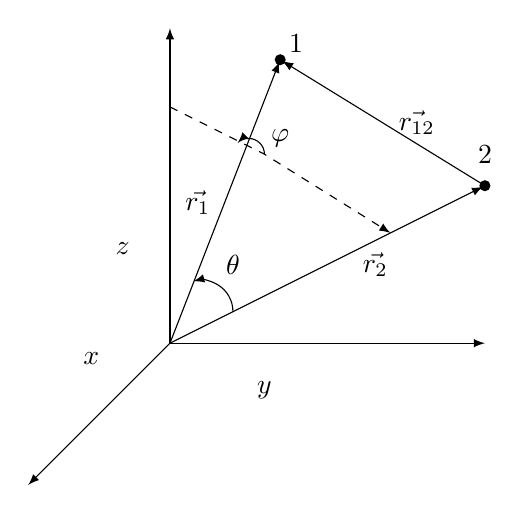
\begin{tikzpicture}[scale=2,inner sep=0,arrows=-latex]
		\draw  (0,0)--(0,2);
		\draw (0,0)--(-0.9,-0.9);
		\draw (0,0)--(2,0);
		\node (x) at (-0.5,-0.1) {\bf $x$};
		\node (y) at (0.6,-0.3) {\bf $y$};
		\node (z) at (-.3,0.6) {\bf $z$};
		% \draw (2,1) circle[radius=0.3];
		\node (A) at (2,1) {};
		\node (i) at (.7,1.8) {} ;
		\node (r1) at (2,1.2) {\bf $2$};
		\node (r2) at (.8,1.9) {\bf $1$} ;
		\fill (i) circle(1pt) ;
		\fill (A) circle(1pt) ;
		\draw (0,0)--node[right=13pt]{${\vec{{r_2}}}$}(A);
		\draw (0,0)--node[left=5pt]{${\vec{{r_1}}}$}(i);
		\draw (A)--node[right=.2cm]{${\vec{{r_{12}}}}$}(i);
		\draw [dashed,] (0,1.5) -- (.6,1.2) -- (1.4,0.7);
		\draw (0.6,1.2) arc (0:135:0.1);
		\node (phi) at (.7,1.3) {$\varphi$} ;
		% \draw[dashed] (0.1,0.05) -- (0.12,.2) -- (0.14,0.36);
		\draw (0.4,0.2) arc (0:105:0.2);
		\node (theta) at (.4,.5) {$\theta$} ;
	\end{tikzpicture}
	% \caption{分子坐标系}
	\label{figA.-1}
\end{figure}
